\documentclass[aspectratio=1610]{beamer}
\usepackage[UKenglish]{datetime}
\usepackage{tikz}
\usepackage{xcolor}
\usepackage{sourcecodepro}
\usepackage[subpreambles]{standalone}
\usepackage{pbox}
\usepackage{listings}
\usepackage{fontspec}

% The Tableau20 colours
\definecolor{TabLightOrange}{RGB}{255,187,120}
\definecolor{TabOrange}{RGB}{255,127,14}
\definecolor{TabLightBlue}{RGB}{174,199,232}
\definecolor{TabBlue}{RGB}{31,119,180}
\definecolor{TabGreen}{RGB}{44,160,44}
\definecolor{TabLightGreen}{RGB}{152,223,138}
\definecolor{TabSalmon}{RGB}{255,152,150}
\definecolor{TabRed}{RGB}{214,39,40}
\definecolor{TabPurple}{RGB}{148,103,189}
\definecolor{TabLightPurple}{RGB}{197,176,213}
\definecolor{TabLightPink}{RGB}{247,182,210}
\definecolor{TabPink}{RGB}{227,119,194}
\definecolor{TabLightBrown}{RGB}{196,156,148}
\definecolor{TabBrown}{RGB}{140,86,75}
\definecolor{TabGray}{RGB}{127,127,127}
\definecolor{TabOlive}{RGB}{188,189,34}
\definecolor{TabLightOlive}{RGB}{219,219,141}
\definecolor{TabLightGray}{RGB}{199,199,199}
\definecolor{TabLightCyan}{RGB}{158,218,229}
\definecolor{TabCyan}{RGB}{23,190,207}

\setmainfont{Inter}
% \usepackage[scaled=0.96,osf,tighter]{newpxtext}
% \linespread{1.05} % Maintain 12pt line spacing
\usecolortheme[named=TabBlue]{structure}

\titlegraphic{%
  \vspace{0.5cm}
  
\includegraphics[width=3cm,keepaspectratio]{../assets/tarides.png}
}

\setbeamercolor{block title alerted}{fg=TabRed,bg=white}
\setbeamercolor{block body alerted}{fg=black,bg=white}
\setbeamercolor{alerted text}{fg=TabRed}

\makeatletter
\tikzset{
  dot diameter/.store in=\dot@diameter,
  dot diameter=3pt,
  dot spacing/.store in=\dot@spacing,
  dot spacing=10pt,
  dots/.style={
    line width=\dot@diameter,
    line cap=round,
    dash pattern=on 0.5pt off \dot@spacing
  }
}
\makeatother

\usetikzlibrary{positioning}
\usetikzlibrary{calc}
\usetikzlibrary{shapes.geometric}
\usetikzlibrary{backgrounds}

\newdateformat{withoutyearformat}{%
  \dayofweekname{\THEDAY}{\THEMONTH}{\THEYEAR}\ %
  \ordinal{DAY}\ %
  \monthname[\THEMONTH]%
}
\withoutyearformat

\usefonttheme{serif}
\setbeamerfont{title}{family=\fontspec{Inter}, size=\huge}
\setbeamerfont{frametitle}{family=\fontspec{Inter},shape=\bfseries}
\setbeamertemplate{headline}{}
\setbeamertemplate{footline}[frame number]{}
\setbeamertemplate{navigation symbols}{} %remove navigation symbols

\setbeamertemplate{caption}{\raggedright\insertcaption\par}

\lstset{
  tabsize=2,
  showspaces=false,
  showstringspaces=false,
  basicstyle=\normalsize\ttfamily,
  breaklines=true,
}

\let\otp\titlepage
\renewcommand{\titlepage}{\otp\addtocounter{framenumber}{-1}}

\newcommand\Wider[2][3em]{%
  \makebox[\linewidth][c]{%
    \begin{minipage}{\dimexpr\textwidth+#1\relax}
      \raggedright#2
    \end{minipage}%
  }%
}

\newcommand{\backupbegin}{
  \newcounter{framenumberappendix}
  \setcounter{framenumberappendix}{\value{framenumber}}
}
\newcommand{\backupend}{
  \addtocounter{framenumberappendix}{-\value{framenumber}}
  \addtocounter{framenumber}{\value{framenumberappendix}} 
}

\def\gitcolorblack{\color{black}}
\def\gitcolorred{\color{TabRed}}
\def\gitcolorgreen{\color{TabGreen}}
\def\gitcoloryellow{\color{TabPurple}}
\def\gitcolorblue{\color{TabBlue}}
\def\gitcolormagenta{\color{TabPink}}
\def\gitcolorcyan{\color{TabCyan}}
\def\gitcolorwhite{\color{white}}

\title[TraceRPC]{\textsc{\textbf{%
      {\fontsize{2em}{2.5em}\selectfont C}%
      {\fontsize{1.6em}{2.5em}\selectfont AUSAL}%
      {\fontsize{2em}{2.5em}\selectfont RPC}}}}
\subtitle{\large \emph{Distributed computation over Irmin}}
\author{Craig Ferguson (\texttt{@CraigFe})}
\date{\\[-1.5cm]\formatdate{23}{8}{2019}}

\begin{document}

\maketitle

\begin{frame}{Remote Procedure Call (RPC)}

  \begin{center}
    Remote computation at the level of individual function calls.\vspace{5mm}
    \includestandalone[width=0.9\textwidth]{../diagrams/architecture}
  \end{center}
\end{frame}

\begin{frame}{Trendy microservice architectures}
  \begin{center}
  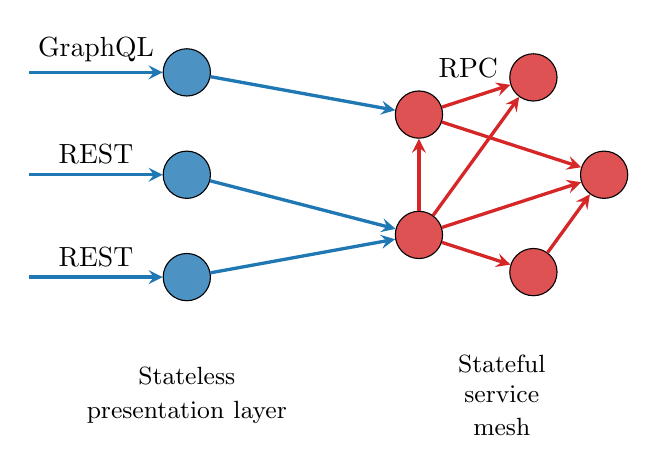
\begin{tikzpicture}[
    n/.style = {
      , circle
      , minimum size = 0.6cm
      , inner sep = 0pt
      , draw = black
    }
    , web/.style = {
      n,
      fill=TabBlue!80
    }
    , service/.style = {
      n,
      fill=TabRed!80
    }
    , state/.style = {
      n,
      fill=TabRed!80
    }
    , incarrow/.style = {
      , ->
      , >=stealth
      , draw=TabBlue
      , very thick
    }
    , statearrow/.style = {
      incarrow,
      draw=TabRed
    }
    , biglabel/.style = {
      , text width=3cm
      , text centered
    }
    , on grid
    , node distance = 1.3cm
    ]
    \node[web] (web1) {};
    \node[web, below = of web1] (web2) {};
    \node[web, below = of web2] (web3) {};
    % \node[below = of web3] (web-ellipsis) {\huge $...$};
    \node[below = 1.5cm of web3, biglabel] (label1) {\small Stateless\\ presentation layer};

    \coordinate[right = 4cm of web2] (center);
    \coordinate (label2) at (center |- 0, 0 |- label1);

    \node[biglabel] at (label2) {\small Stateful\\ service\\ mesh};

    \def\leftarrowsep{2}
    \def\radius{1.3cm}
    \def\extradius{2.4cm}
    \def\angle{180+36}

    \draw[incarrow] ($ (web1) + (-\leftarrowsep, 0) $) -- node[above] {GraphQL} (web1);
    \draw[incarrow] ($ (web2) + (-\leftarrowsep, 0) $) -- node[above] {REST} (web2);
    \draw[incarrow] ($ (web3) + (-\leftarrowsep, 0) $) -- node[above] {REST} (web3);

    
    \node[service] at ($ (center) + (\angle+0:\radius) $) (s1) {};
    \node[service] at ($ (center) + (\angle+72:\radius) $) (s2) {};
    \node[service] at ($ (center) + (\angle+144:\radius) $) (s3) {};
    \node[service] at ($ (center) + (\angle+216:\radius) $) (s4) {};
    \node[service] at ($ (center) + (\angle+288:\radius) $) (s5) {};

    \draw[incarrow] (web1) -- (s5);
    \draw[incarrow] (web2) -- (s1);
    \draw[incarrow] (web3) -- (s1);
    
    \draw[statearrow] (s1) -- (s2);
    \draw[statearrow] (s1) -- (s5);
    \draw[statearrow] (s2) -- (s3);
    \draw[statearrow] (s5) -- node[above, xshift=-1mm, yshift=1mm] {RPC} (s4);
    
    \draw[statearrow] (s1) -- (s4);
    \draw[statearrow] (s1) -- (s3);
    \draw[statearrow] (s5) -- (s3);
  \end{tikzpicture}
  \vspace{6mm}
  
  Use RPC for remote access to a resource (storage, private network etc.).
  \end{center}
  % These concurrency control mechanisms are particularly problematic for RPC, since RPC
  % encourages you to think of it like a local function call; so it needs to be low latency
  % and low cost.
\end{frame}

% \begin{frame}{Overview}
%   \begin{center}
%     \begin{tikzpicture}[
%       state/.style =
%       { rectangle
%         , rounded corners
%         , draw=black
%         , very thick
%         , minimum height=2em
%         , inner sep=2pt
%         , text centered
%       }
%       , arrow/.style =
%       { very thick
%         , ->
%         , >=stealth
%       }
%       ]

%       \node[state] (problem) {RPC contention};
%       \node[state, below = of problem] (irmin) {Irmin};
%       \node[state, right = of problem] (mergerpcs) {
%         \begin{tabular}{c}
%           Mergeable\\RPCs
%           \end{tabular}
%       };
      
%       \draw[arrow] (problem) -- (mergerpcs);
%       \draw[arrow] (irmin) -- (mergerpcs);
%     \end{tikzpicture}
%   \end{center}
% \end{frame}

\begin{frame}{Two birds and one cannonball}

  \pause

  \begin{alertblock}{\\[-2mm]\hspace{1mm}\textbf{Problem:} consistency under race conditions}
    \begin{itemize}
    \item[--] breaks RPC abstraction
    \item[--] results in additional round-trips to server
    \end{itemize}
  \end{alertblock}

  \pause

  \begin{alertblock}{\\[-2mm]\hspace{1mm}\textbf{Problem:} tracing distributed
      systems}
    \begin{itemize}
    \item[--] neither the middleware nor the application layer has full context
    \item[--] linear log outputs on remote systems must be correlated
    \end{itemize}
  \end{alertblock}

  \vspace{3mm}
  \pause
  \begin{exampleblock}{\\[-2mm]\hspace{1mm}\textbf{Idea:} middleware that
      understands state\vspace{1mm}}
    \begin{itemize}
    \item[--] application explains the underlying state to
      the middleware
    \item[--] middleware resolves conflicts and constructs a trace as
      it goes
    \end{itemize}
    % In particular, we'd like the middleware to provide a consistency model such that the trace
    % makes it easy for us to reason about the _intent_ of the 
  \end{exampleblock}

\end{frame}

\begin{frame}{Introducing Irmin}
  \begin{itemize}
  \item Distributed, immutable Merkle trees with push/pull sync -- just like Git!\vspace{2mm}
  \item Pure OCaml; unikernel-compatible.\vspace{2mm}
  \item Parameterised on:\vspace{1mm}
    \begin{itemize}
    \item Storage backend (Memory, FS, Git repo, Redis, ...)\vspace{1mm}
    \item User-defined mergable contents (leaves of the tree)
    \end{itemize}
  \end{itemize}

  % \begin{lstlisting}
  %   module Typ

  % % \end{lstlisting}
  % \begin{tikzpicture}
  %   % \node
  %   \end{tikzpicture}

\end{frame}

\begin{frame}{Aside: why \underline{\emph{three}}-way merge?}
  \pause
  % When writing a CRDT, you often find you need to push more contextual information into the type
  % to compensate for the lack of context provided as a baseline. Irmin (and by extension,
  % CausalRPC) goes for the more heavy-weight approach of providing causal consistency as a
  % baseline, and the user can choose to strengthen % the consistency model when they want in
  % the design of their merge operation.
  \begin{center}
  \begin{tabular}{c c c}
    \emph{Two}-way CRDT\textsuperscript{1} merge &\quad\quad\quad & \onslide<3->{\emph{Three}-way Irmin merge\vspace{0.5cm}} \\
    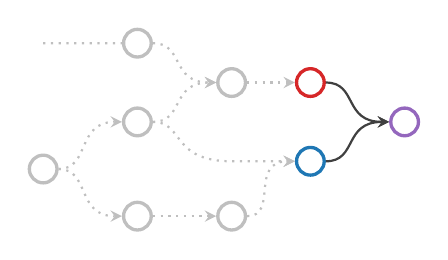
\begin{tikzpicture}[
      , commit/.style={circle,draw,very thick, inner sep = 0pt, minimum size=10pt}
      , c-out/.style={color=TabPurple}
      , on grid
      ]

      \tikzset{>=stealth}

      \node[commit, color=TabRed] (in1) {};
      \node[commit, color=TabBlue, below = of in1] (in2) {};
      \coordinate (in-middle) at ($ (in1)!0.5!(in2) $);

      \node[commit, color=lightgray, left = of in1] (is2) {};

      \coordinate (left-middle) at (is2 |- 0, 0 |- in-middle);
      \coordinate (left-bottom) at (is2 |- 0, 0 |- in2);
      \node[commit, color=lightgray, below = 0.5cm of left-bottom] (unknown-bottom) {};

      \node[commit, color=lightgray, left = of left-middle] (lca) {};
      \node[commit, color=lightgray, above = of lca] (unknown-top) {};
      \node[commit, c-out, right = of in-middle] (out) {};

      \node[commit, color=lightgray] (unknown-bottom-arrow) at (lca |- 0, 0 |- unknown-bottom) {};

      \coordinate (bar) at ($ (lca)!0.5!(unknown-bottom-arrow) $);
      \node[commit, color=lightgray, left = 1cm of bar] (foo) {};
      
      \draw[->, color=lightgray, thick, dotted] (unknown-bottom-arrow) -- (unknown-bottom);
      \draw[->, color=lightgray, thick, dotted] (is2) -- (in1);

      \def\bezx{0.6}
      \draw[->, color=lightgray, thick, dotted] (foo) .. controls +(\bezx,0) and +(-1.3*\bezx,0) .. (lca);
      \draw[->, color=lightgray, thick, dotted] (foo) .. controls +(\bezx,0) and +(-1.3*\bezx,0) .. (unknown-bottom-arrow);
      
      \draw[->, color=lightgray, thick, dotted] (unknown-bottom) .. controls +(\bezx,0) and +(-1.3*\bezx,0) .. (in2);

      \coordinate (unknown-top-foo) at (foo |- 0, 0 |- unknown-top);
      \draw[->, color=lightgray, thick, dotted] (unknown-top-foo) -- (unknown-top) .. controls +(\bezx,0) and +(-1.3*\bezx,0) .. (is2);
      \draw[->, color=lightgray, thick, dotted] (lca) .. controls +(\bezx,0) and +(-1.3*\bezx,0) .. (left-bottom) -- (in2);
      \draw[->, color=lightgray, thick, dotted] (lca) .. controls +(\bezx,0) and +(-1.3*\bezx,0) .. (is2);

      \draw[->, color=darkgray, thick] (in1) .. controls +(\bezx,0) and +(-1.3*\bezx,0) .. (out);
      \draw[->, color=darkgray, thick] (in2) .. controls +(\bezx,0) and +(-1.3*\bezx,0) .. (out);
    \end{tikzpicture}
                                                                          & &
    \onslide<3->{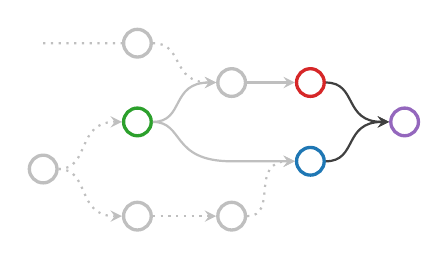
\begin{tikzpicture}[
      , commit/.style={circle,draw,very thick, inner sep = 0pt, minimum size=10pt}
      , c-out/.style={color=TabPurple}
      , on grid
      ]

      \tikzset{>=stealth}

      \node[commit, color=TabRed] (in1) {};
      \node[commit, color=TabBlue, below = of in1] (in2) {};
      \coordinate (in-middle) at ($ (in1)!0.5!(in2) $);

      \node[commit, color=lightgray, left = of in1] (is2) {};

      \coordinate (left-middle) at (is2 |- 0, 0 |- in-middle);
      \coordinate (left-bottom) at (is2 |- 0, 0 |- in2);
      \node[commit, color=lightgray, below = 0.5cm of left-bottom] (unknown-bottom) {};

      \node[commit, color=TabGreen, left = of left-middle] (lca) {};
      \node[commit, color=lightgray, above = of lca] (unknown-top) {};
      \node[commit, c-out, right = of in-middle] (out) {};

      \node[commit, color=lightgray] (unknown-bottom-arrow) at (lca |- 0, 0 |- unknown-bottom) {};

      \coordinate (bar) at ($ (lca)!0.5!(unknown-bottom-arrow) $);
      \node[commit, color=lightgray, left = 1cm of bar] (foo) {};
      
      \draw[->, color=lightgray, thick, dotted] (unknown-bottom-arrow) -- (unknown-bottom);
      \draw[->, color=lightgray, thick] (is2) -- (in1);

      \def\bezx{0.6}
      \draw[->, color=lightgray, thick, dotted] (foo) .. controls +(\bezx,0) and +(-1.3*\bezx,0) .. (lca);
      \draw[->, color=lightgray, thick, dotted] (foo) .. controls +(\bezx,0) and +(-1.3*\bezx,0) .. (unknown-bottom-arrow);
      
      \draw[->, color=lightgray, thick, dotted] (unknown-bottom) .. controls +(\bezx,0) and +(-1.3*\bezx,0) .. (in2);

      \coordinate (unknown-top-foo) at (foo |- 0, 0 |- unknown-top);
      \draw[->, color=lightgray, thick, dotted] (unknown-top-foo) -- (unknown-top) .. controls +(\bezx,0) and +(-1.3*\bezx,0) .. (is2);
      \draw[->, color=lightgray, thick] (lca) .. controls +(\bezx,0) and +(-1.3*\bezx,0) .. (left-bottom) -- (in2);
      \draw[->, color=lightgray, thick] (lca) .. controls +(\bezx,0) and +(-1.3*\bezx,0) .. (is2);

      \draw[->, color=darkgray, thick] (in1) .. controls +(\bezx,0) and +(-1.3*\bezx,0) .. (out);
      \draw[->, color=darkgray, thick] (in2) .. controls +(\bezx,0) and +(-1.3*\bezx,0) .. (out);
    \end{tikzpicture} \vspace{0.5cm}}
    \\
    $\text{\small\textcolor{TabRed}{\normalfont state}} \rightarrow
    \text{\small\textcolor{TabBlue}{state}} \rightarrow
    \text{\small\textcolor{TabPurple}{state}}$ & &

    \onslide<3->{$\textsf{\textcolor{TabGreen}{lca\,:\,state}} \rightarrow \textsf{\textcolor{TabRed}{state}} \rightarrow \textsf{\textcolor{TabBlue}{state}}
    \rightarrow \textsf{\textcolor{TabPurple}{state}}$} \\
  \end{tabular}
\end{center}
  % \begin{itemize}
  % \item \textcolor{TabGreen}{+ve: easier to use (additional context of intent)}
  % \item \textcolor{TabRed}{--ve: tracing overhead (explicit causal history tracking)}
  % \end{itemize}
\vspace{0.5cm}
\onslide<3->{\textcolor{TabGreen}{Lowest common ancestor} allows the merge operation to reason about
  \emph{intent}.}

\vspace{1cm}
\small\textsuperscript{1}{\footnotesize M.~Shapiro et al. \emph{Conflict-Free Replicated Data
    Types}, 2011.}
\end{frame}

\begin{frame}{State-aware RPC}
  \begin{center}
    \includestandalone[width=\textwidth]{../diagrams/layering}
  \end{center}
\end{frame}

\begin{frame}{The life of an RPC thread}
  \begin{center}
    \includestandalone[width=\textwidth]{../diagrams/fsm}
    \vspace{0.5cm}
  \end{center}
\end{frame}

% \begin{frame}{The interface}
% \begin{center}
% \begin{tabular}{l}
% \begin{lstlisting}
% module MakeServer 
%   (B: BACKEND)                             (* Unix FS / Unix Mem / MirageOS *)
%   (C: CONTENTS)                            (* Base type and merge function *)
%   (Iface: functor (I: IDL) -> IFACE        (* Interface over correct base type *)
%           with type base = C.t)          
%   (Impl:  functor (I: IDL) -> IMPL         (* Matching implementation *)
%           with type shape = Iface.shape): Server
% \end{lstlisting}
% \end{tabular}
% \end{center}
% \end{frame}

\newcommand{\rulesep}{\unskip\ \color{gray75}\vrule width 1.5pt\color{black}}
\definecolor{gray75}{gray}{0.75}
\begin{frame}{Mergeable filesystems}
  \Wider[3em]{
    \begin{center}
      \includestandalone{../diagrams/client-race}
      \ \ \rulesep\ \ %
      \includestandalone{../diagrams/conflict-history}
    \end{center}
  }
\end{frame}

\begin{frame}{Mergeable filesystems: trace output}
  \Wider[2em]{
    \lstinputlisting[nolol=true,escapeinside={[*}{*]}]{../assets/client-race-prompt.txt}
    \pause
    \lstinputlisting[nolol=true,escapeinside={[*}{*]}]{../assets/client-race.txt}
  }
\end{frame}

\begin{frame}{Why OCaml?}
  \textcolor{TabGreen}{\textbf{Portability}} -- Inherits the Mirage mindset towards platform-independence.

  \pause
  \vspace{0.8cm}
  \textcolor{TabGreen}{\textbf{Type-safety}} -- Strict interface definition using an embedded DSL.

  \pause
  \vspace{0.8cm}
  
  \textcolor{TabGreen}{\textbf{Coolness-factor}} \textcolor{TabGray}{(!!!)} -- Protocol design in OCaml is really fun.
\end{frame}


\begin{frame}{Performance: latency}
  \begin{center}
    \Wider[3em]{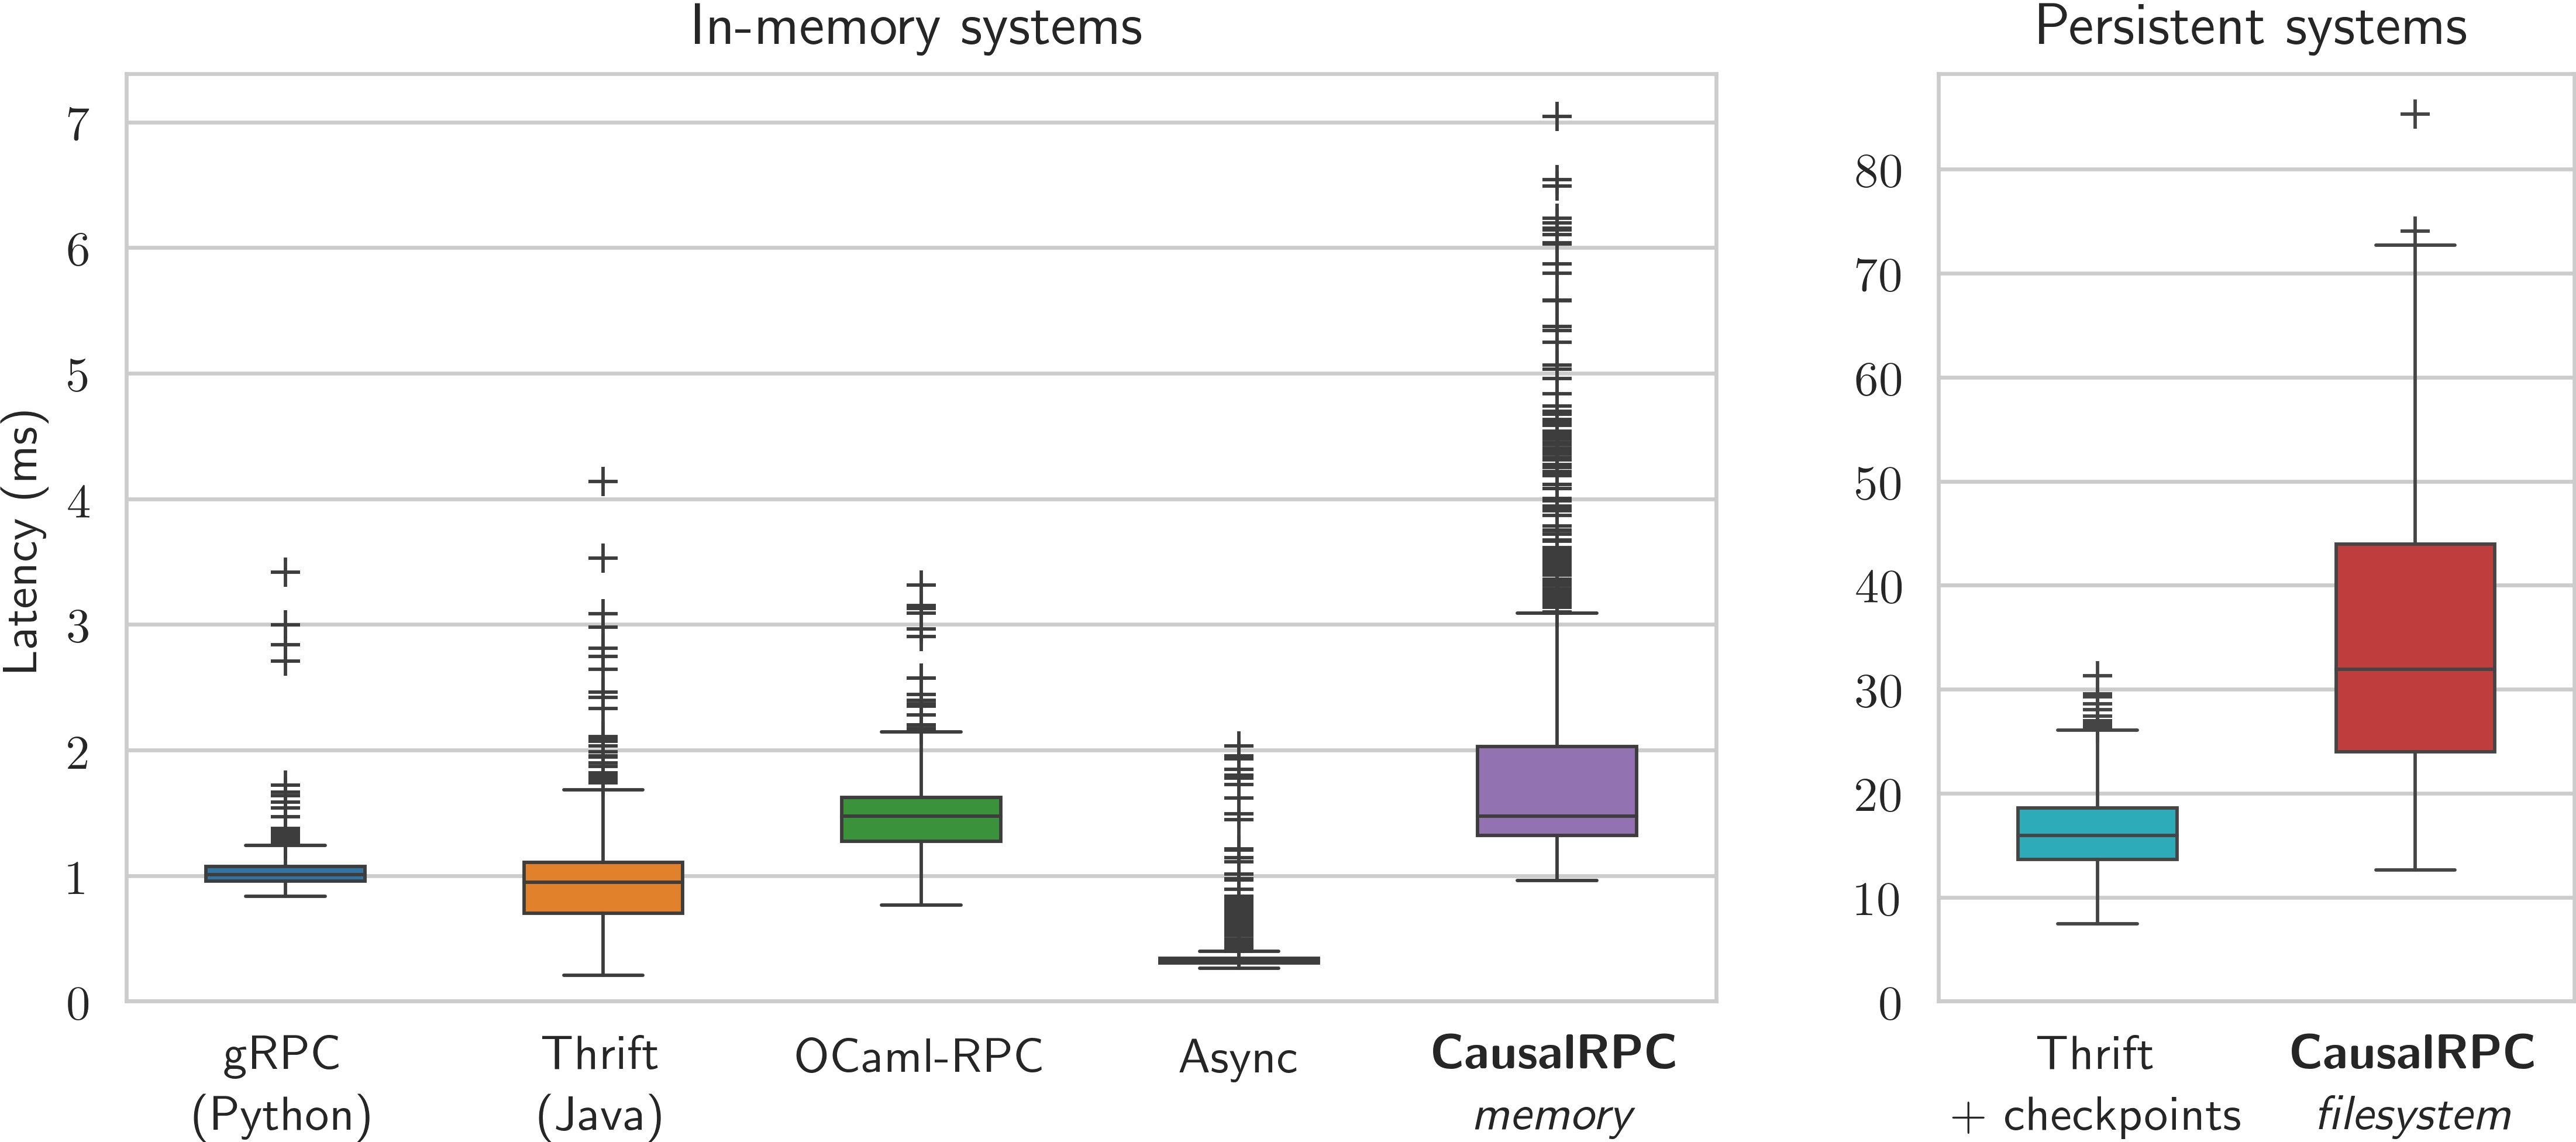
\includegraphics[width=\textwidth]{../assets/latency.png}}
  \end{center}
  \vspace{0.5cm}
  \emph{\footnotesize Measured over 1000 RPCs for a single client-server pair over a Docker bridge
    network.}
\end{frame}

\begin{frame}[t]{}
  \vspace{1mm}
  Server run-time cost profile from first packet receipt to final packet send:
  \vspace{-1mm}
  \begin{center}
    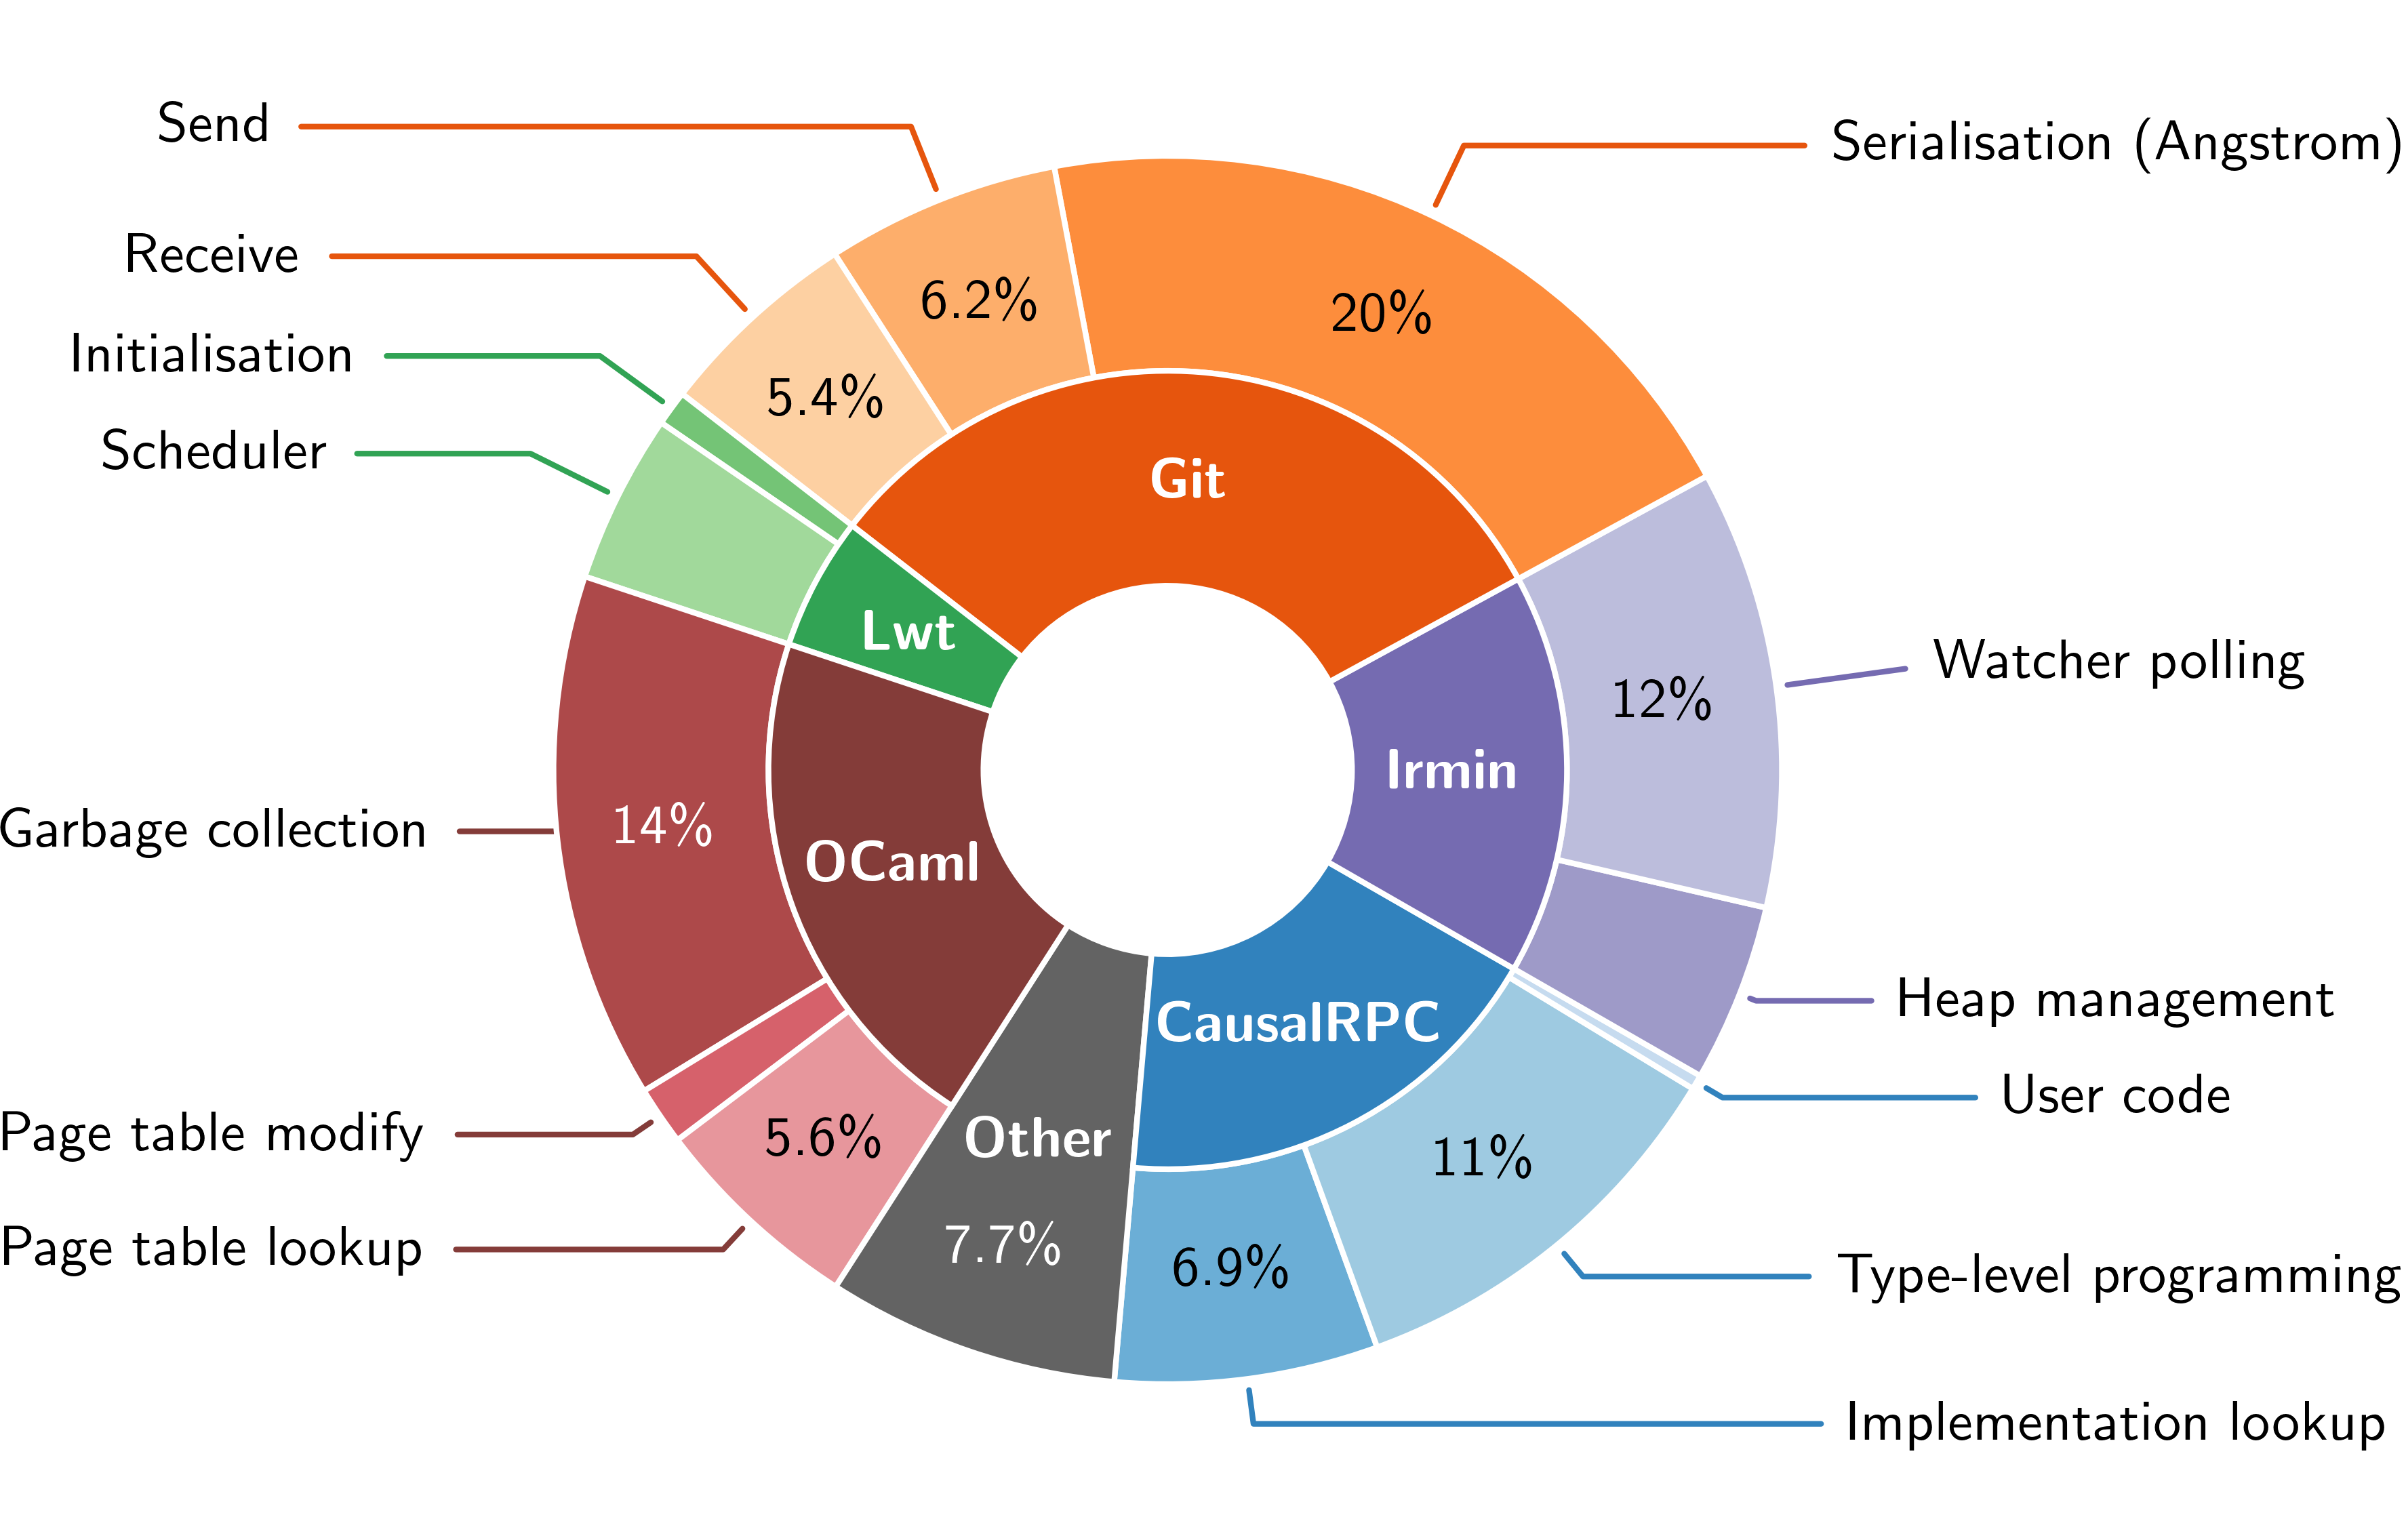
\includegraphics[width=0.94\textwidth]{../assets/piechart.png}\\[-3mm]
    {\scriptsize\textsc{Source}: \emph{\texttt{gprof} and a huge amount of patience.}}
  \end{center}
\end{frame}

\begin{frame}{Performance: memory-usage}
  \begin{center}
    \Wider[3em]{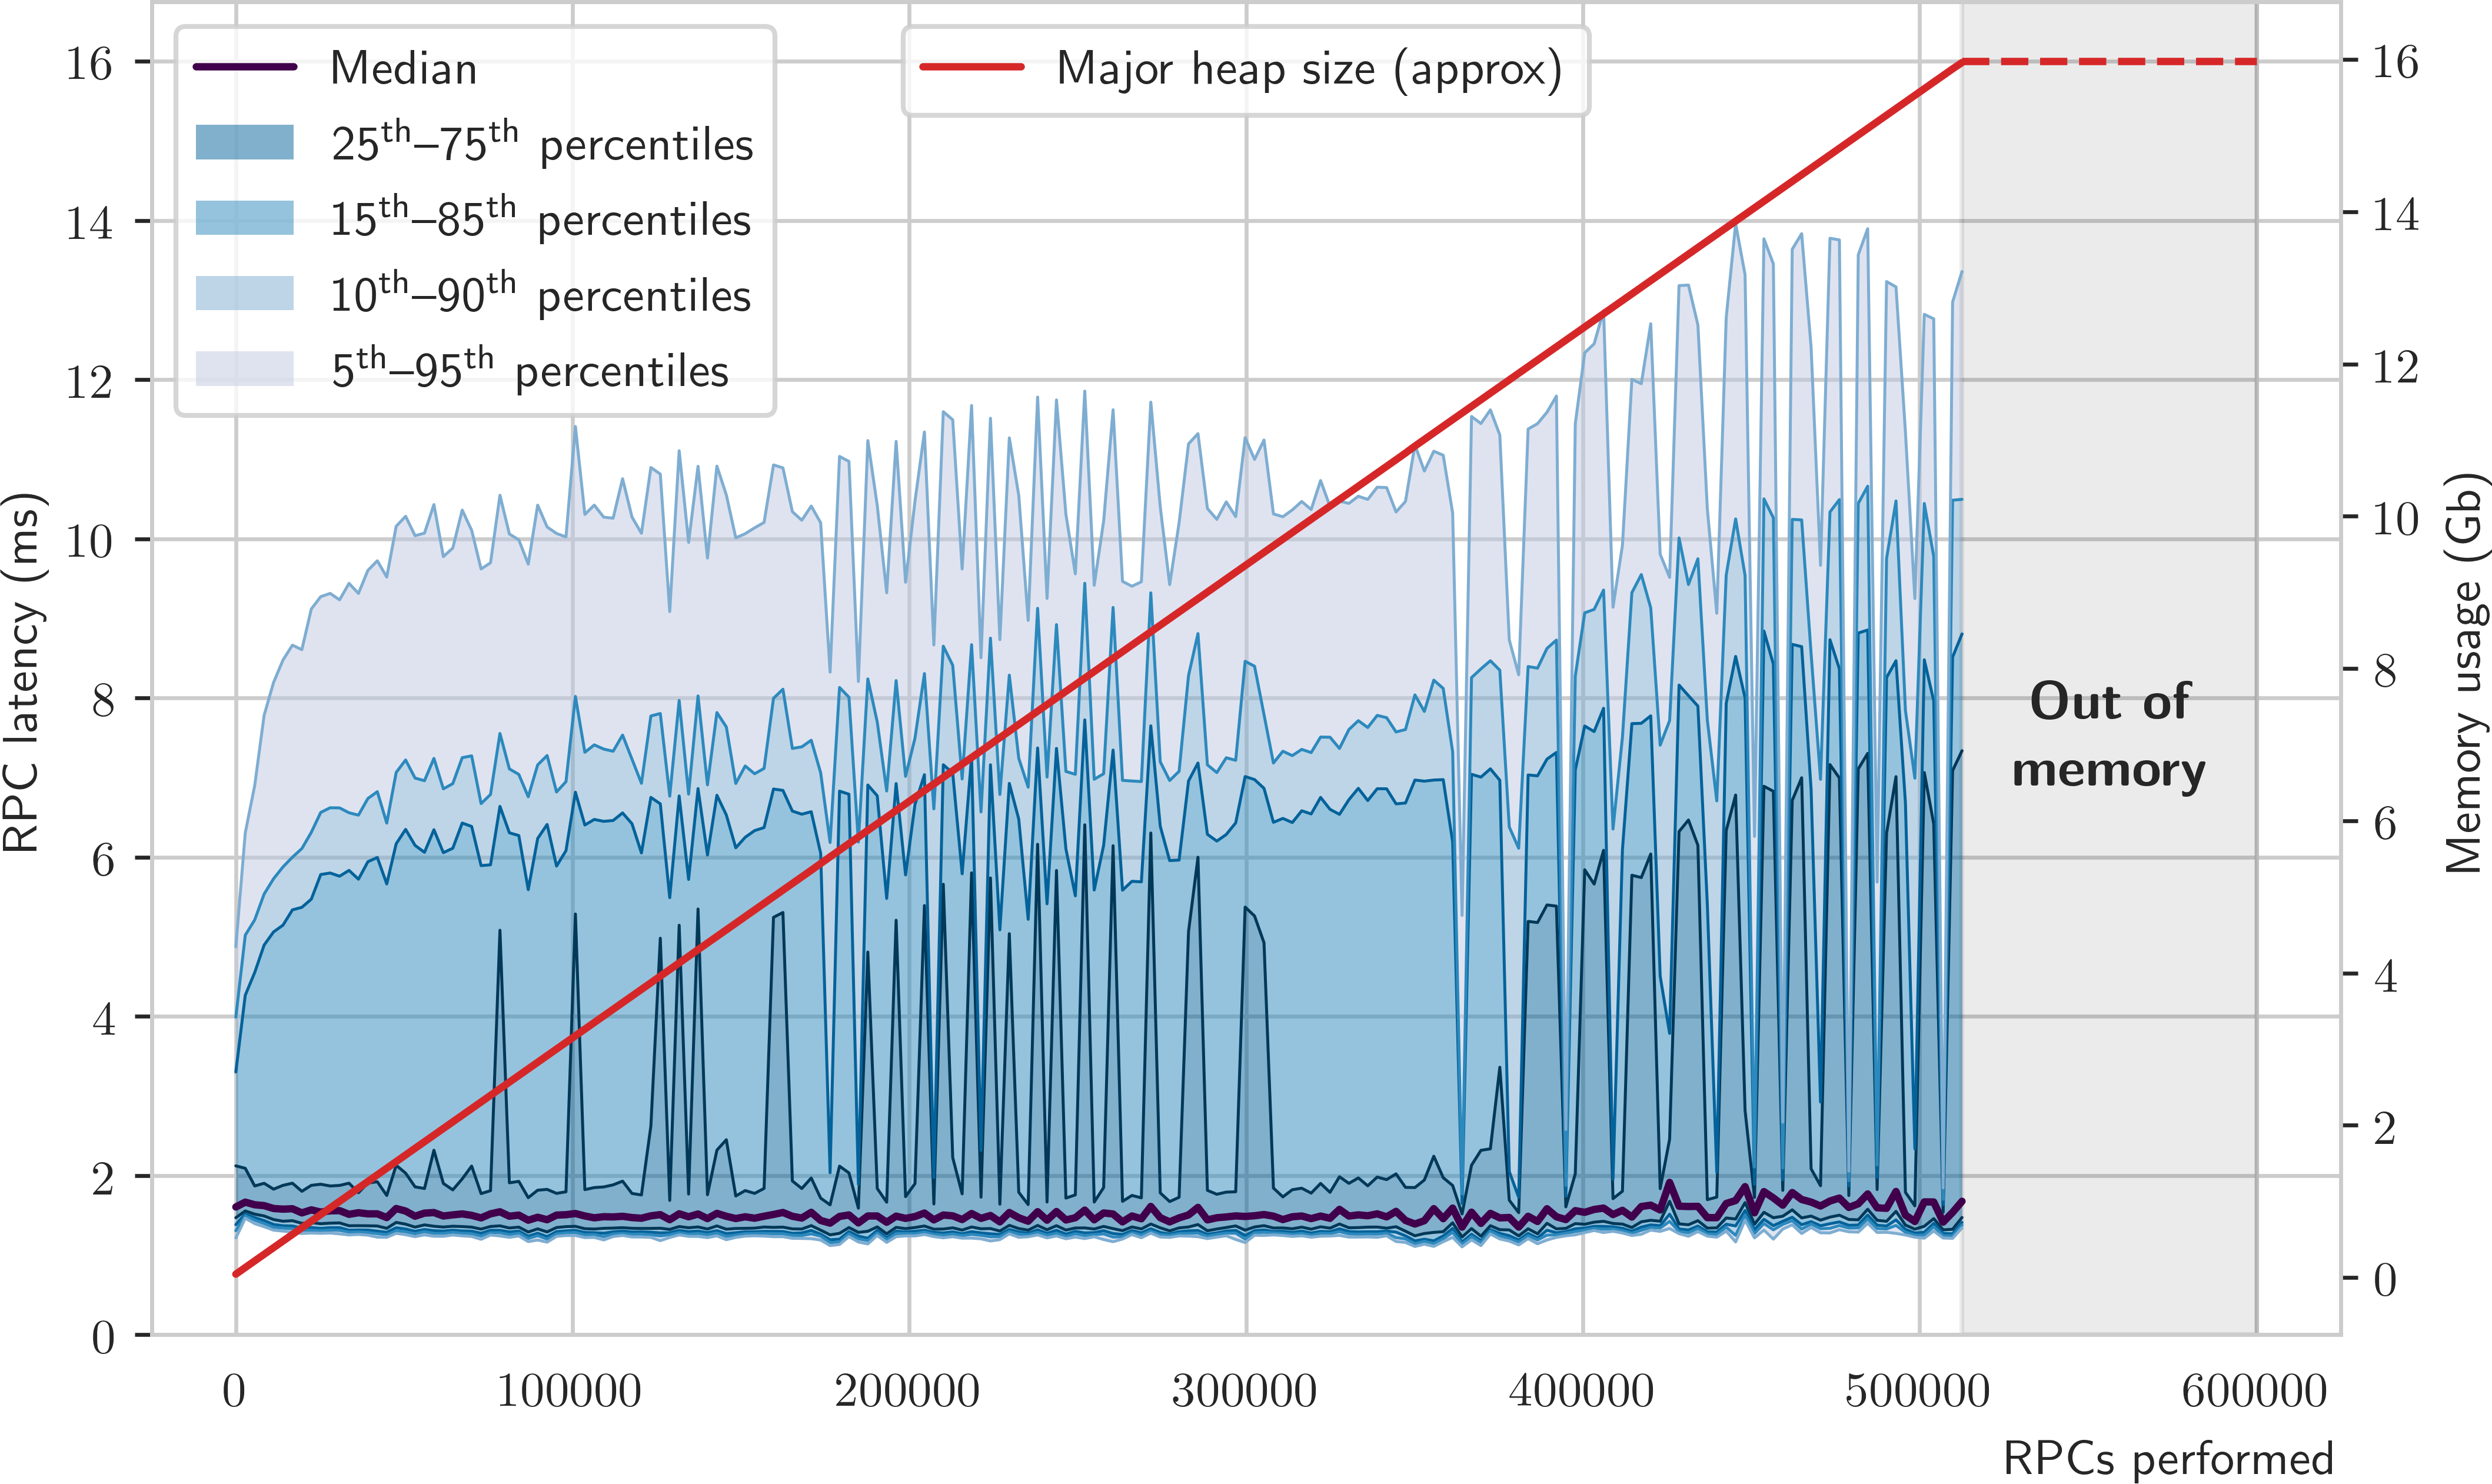
\includegraphics[width=\textwidth]{../assets/latency-mem.png}}
  \end{center}
\end{frame}


\begin{frame}{Generalisation to work clusters}
  \begin{center}
    \pause
    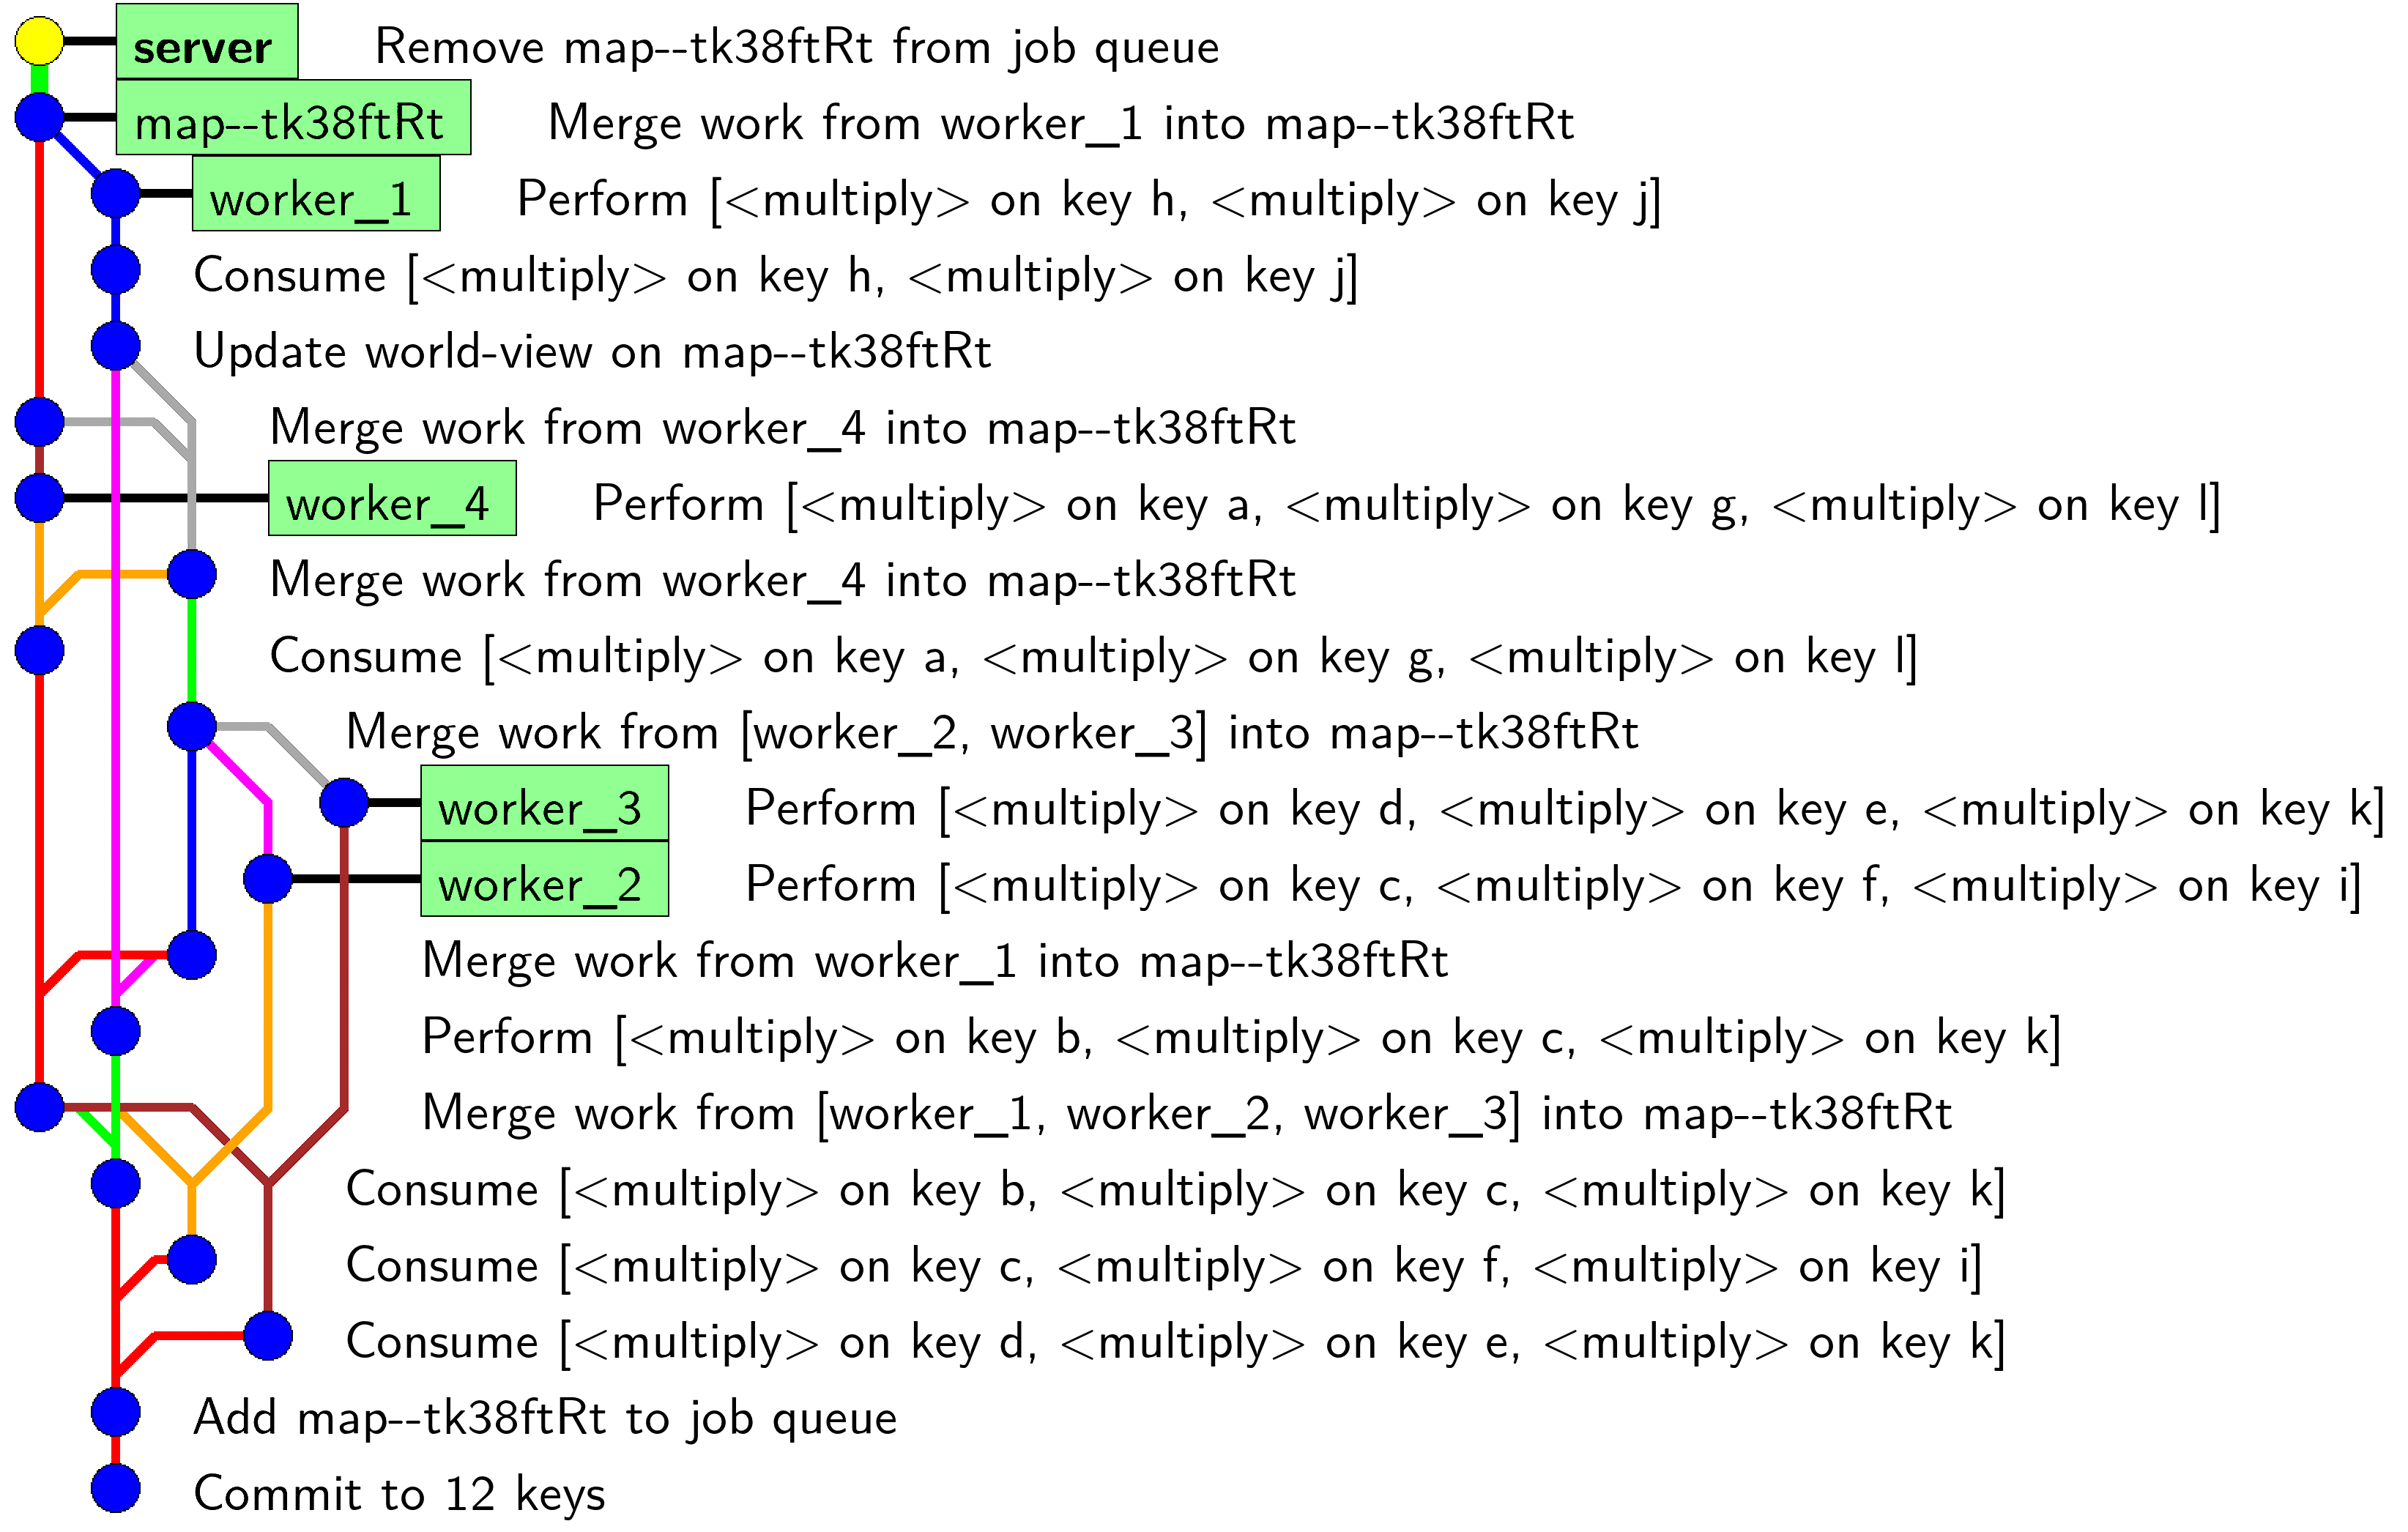
\includegraphics[width=0.95\textwidth]{../assets/gitk.png}
  \end{center}
\end{frame}
  
\begin{frame}{Work cluster scalability}
  Compare cluster performance to Amdahl's law prediction:
  \pause
  \begin{center}
    \Wider[3em]{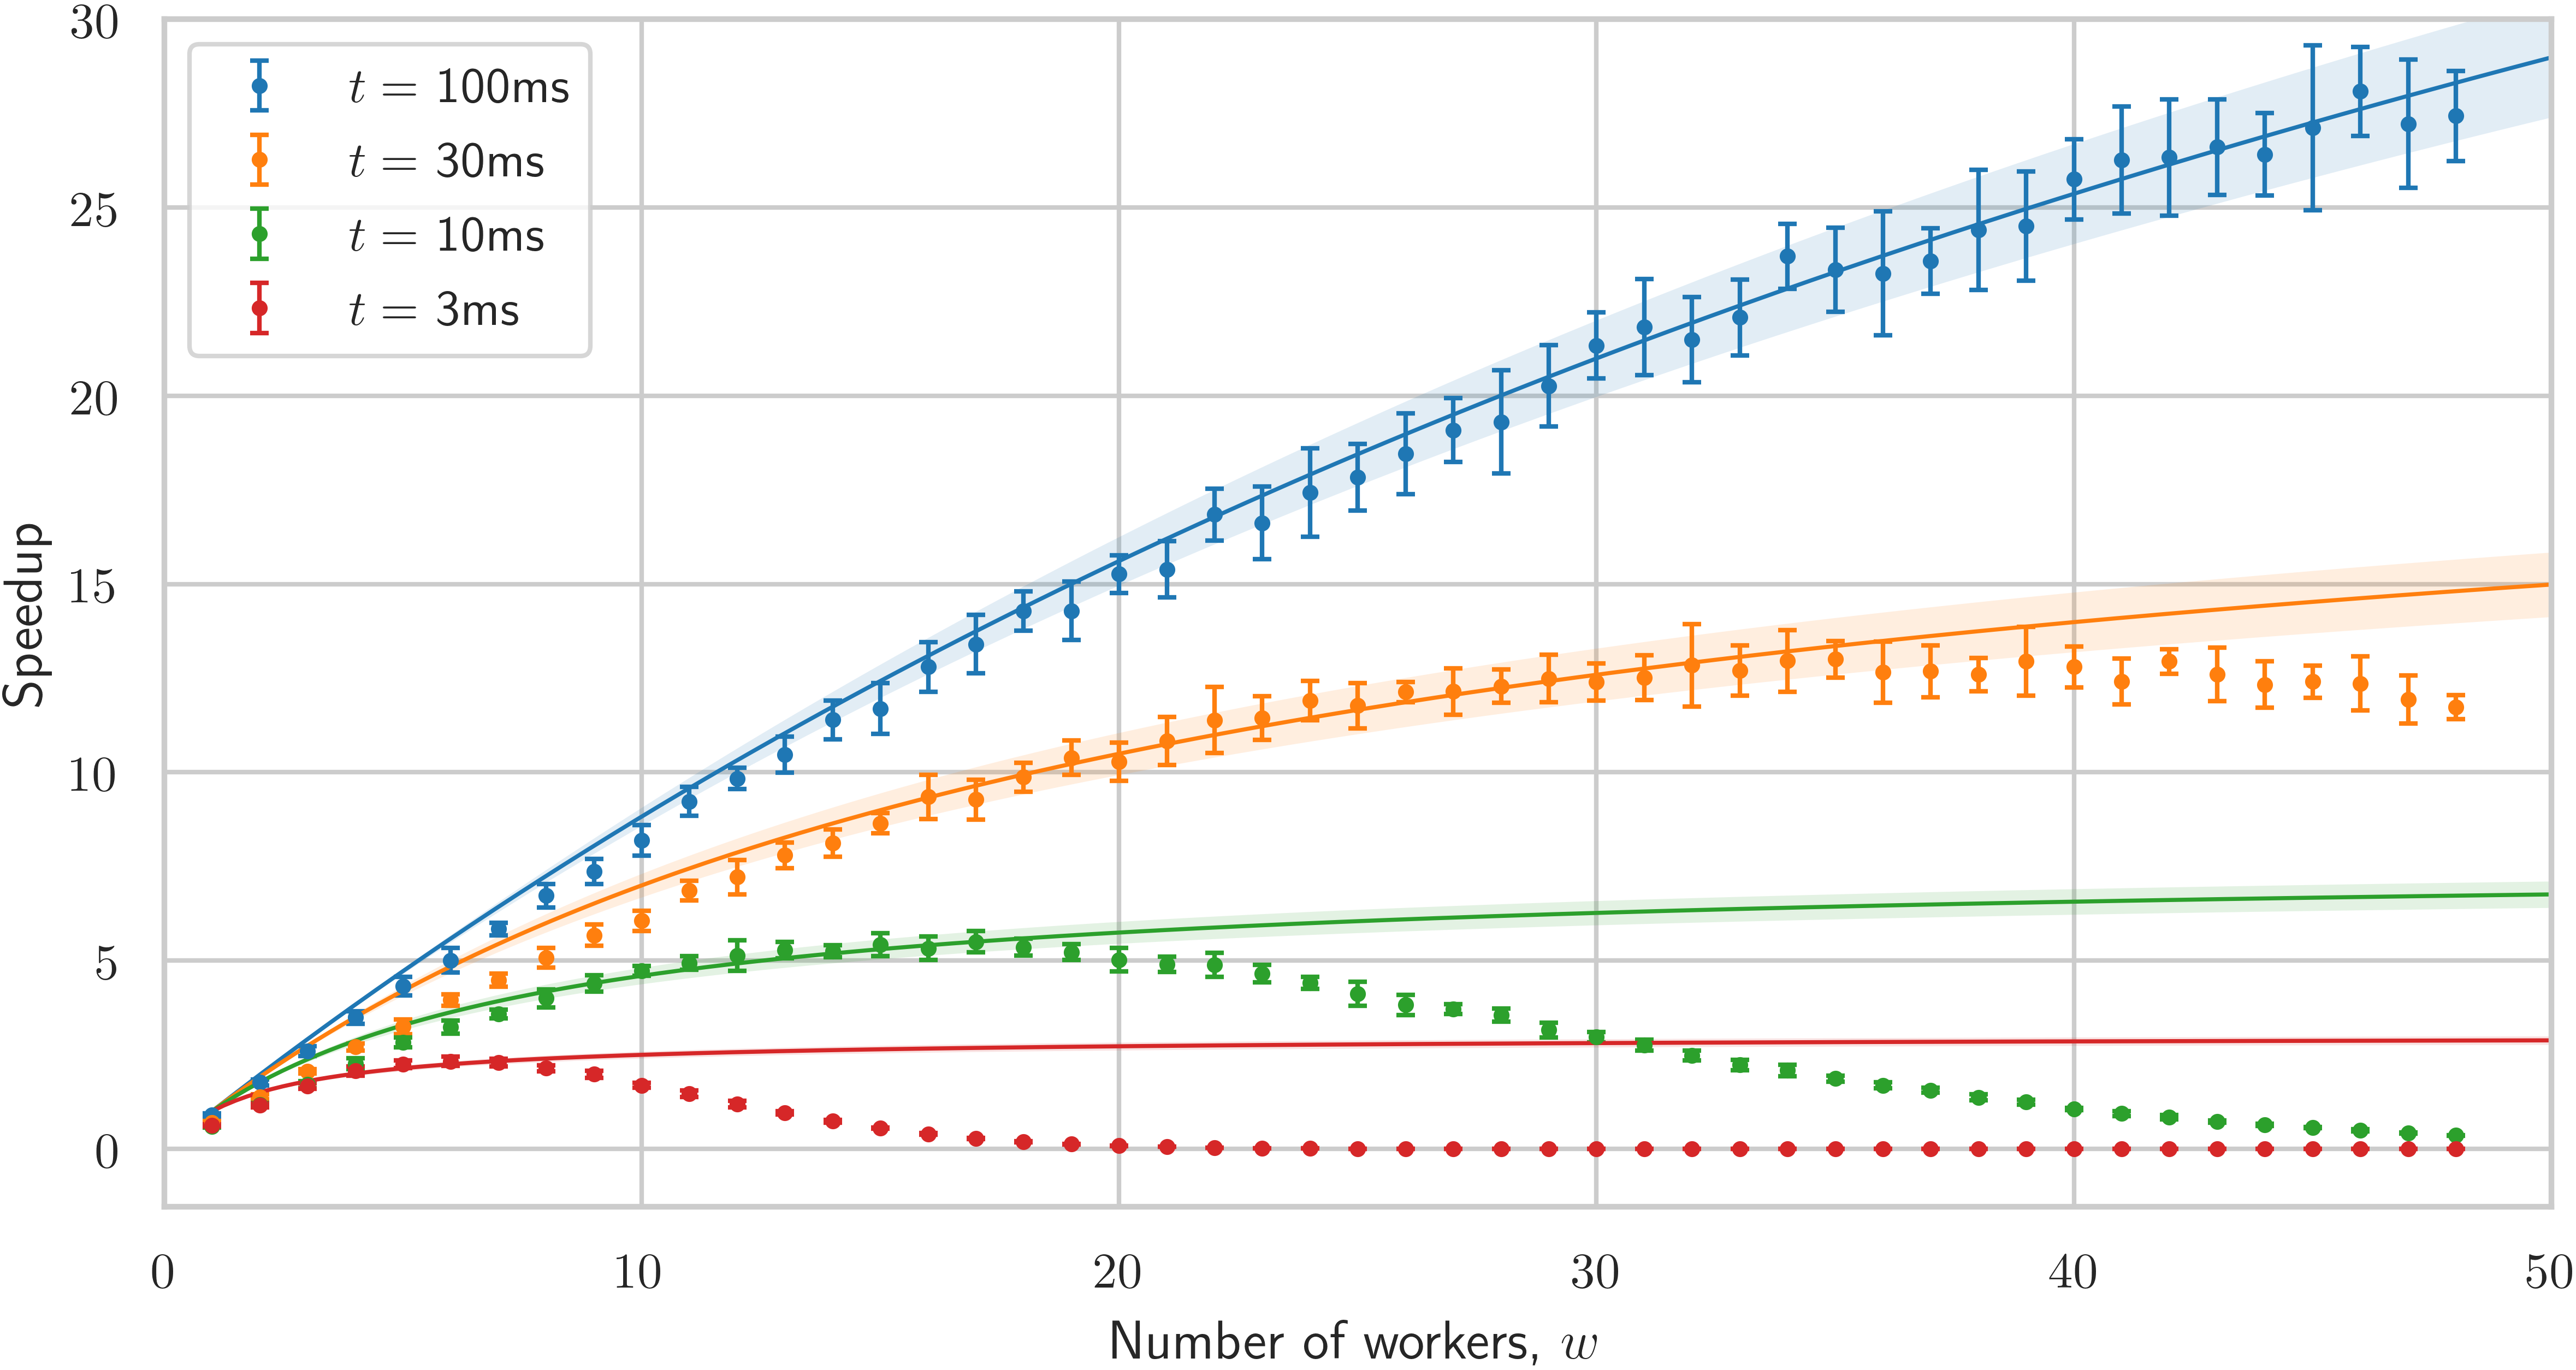
\includegraphics[width=\textwidth]{../assets/amdahl.png}}
  \end{center}
\end{frame}

% \begin{frame}{Extensions: applicative functor interface}

% \end{frame}

\begin{frame}{What next?}
  \begin{center}
    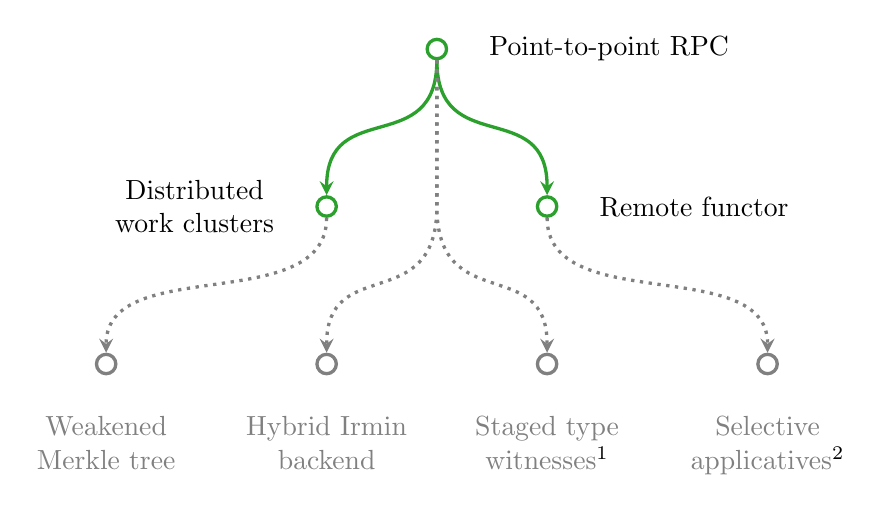
\begin{tikzpicture}
  [ circ/.style= {circle
    , draw
    , very thick
    , inner sep=0pt
    , minimum size=7pt}
  , done/.style={draw=TabGreen}
  , doneish/.style={draw=TabGreen}
  , todo/.style={color=gray}
  , label distance=4mm
  , node distance = 1cm
  , on grid
  ]
  \def\xsep{1.4cm}
  \def\ysep{2cm}
  \def\ybez{1.4}
  \tikzset{>=stealth}

  \onslide<1->{
    \node[circ, done, label=right:{\pbox{10cm}{\relax\ifvmode\centering\fi
        Point-to-point RPC
      }}] (a) at (0,0) {};

    \node[circ, done, below left = \ysep and \xsep of a, label=left:{\pbox{10cm}{\relax\ifvmode\centering\fi
        Distributed \\work clusters
      }}] (b) {};
    \draw[->, very thick, done] (a) .. controls +(0,-\ybez) and +(0,\ybez) .. (b);

    \node[circ, doneish, below right = \ysep and \xsep of a, label=right:{\pbox{10cm}{\relax\ifvmode\centering\fi
        Remote functor
      }}] (c) {};
    \draw[->, very thick, doneish] (a) .. controls +(0,-\ybez) and +(0,\ybez) .. (c);
  }

  \onslide<2->{
    \coordinate (in-middle) at ($ (b)!0.5!(c) $);
    \node[circ, todo, below left = 2*\ysep and \xsep of a, color=gray, label=below:{\pbox{10cm}{\relax\ifvmode\centering\fi
        \textcolor{gray}{Hybrid Irmin}\\\textcolor{gray}{backend}
      }}] (h1) {};
    \draw[->, very thick, color=gray, dotted] (a) -- (in-middle) .. controls +(0,-\ybez) and +(0,\ybez) .. (h1);
  }

  % There's a lot of generic programming holding the IDL together, almost all of which is fully
  % determined at compile time when the Interface and Implementation modules are defined. This is a
  % classic use-case of multistage programming, so we might expect significant performance
  % improvements with that addition.
  \onslide<3->{
    \node[circ, todo, right = 2*\xsep of h1, color=gray, label=below:{\pbox{10cm}{\relax\ifvmode\centering\fi
        \textcolor{gray}{Staged type}\\\textcolor{gray}{witnesses}\textsuperscript{1}
      }}] (h3) {};
    \draw[->, very thick, color=gray, dotted] (a) -- (in-middle) .. controls +(0,-\ybez) and +(0,\ybez) .. (h3);
  }

  \onslide<4->{
    \node[circ, todo, left = 2*\xsep of h1, color=gray, label={below:{\pbox{10cm}{\relax\ifvmode\centering\fi
          \textcolor{gray}{Weakened}\\\textcolor{gray}{Merkle tree}}
      }}] (h2) {};
    \draw[->, very thick, color=gray, dotted] (b) .. controls +(0,-\ybez) and +(0,\ybez) .. (h2);
  }

  \onslide<5->{
    \node[circ, todo, right = 2*\xsep of h3, color=gray, label=below:{\pbox{10cm}{\relax\ifvmode\centering\fi
        \textcolor{gray}{Selective}\\\textcolor{gray}{applicatives}\textsuperscript{2}
      }}] (h4) {};
    \draw[->, very thick, color=gray, dotted] (c) .. controls +(0,-\ybez) and +(0,\ybez) .. (h4);
  }

\end{tikzpicture}
  \end{center}
  \vspace{0.7cm}
  \onslide<3->{\small\textsuperscript{1}{\footnotesize N.~Krishnaswami and J.~Yallop. \emph{A Typed, Algebraic Approach to Parsing}, 2019.}}\\\vspace{2mm}
  \onslide<5->{\small\textsuperscript{2}{\footnotesize A.~Mokhov et al. \emph{Selective Applicative Functors},
    2019.}}
\end{frame}

\begin{frame}{Take-away lessons}
  \begin{enumerate}
  \item \large Simple distributed system abstractions set challenging design constraints.\vspace{3mm}
    \pause
  \item \large Improve semantics by squashing the stack; use OCaml to maintain abstraction and flexibility.\vspace{3mm}
    \pause
  \item \large Consider non-linear log structures in your programs; \emph{casual} logs make it easy to
    reason about intent.
  \end{enumerate}
\end{frame}

\begin{frame}[noframenumbering]
  \begin{center}
    \fontsize{40pt}{50pt}\selectfont \textsc{\textbf{\textcolor{TabBlue}{Thanks For}\\ \textcolor{TabBlue}{Listening}}}
  \end{center}
\end{frame}

\appendix
\backupbegin
\begin{frame}{Related work}
  (Much) more detail in the full dissertation:
  \begin{center}
    \url{https://craigfe.io/out/causalrpc.pdf}
  \end{center}
  \vspace{5mm}

  \textcolor{TabBlue}{mergeable types}
  \begin{itemize}
  \item Conflict-free replicated datatypes. [M.~Shapiro et al. 2011]
  \item Mergeable types. [B~Farinier et al. 2015]
  \end{itemize}
  \vspace{5mm}

  \textcolor{TabBlue}{embedded DSLs for RPC}
  \begin{itemize}
  \item Pickler combinators. [A. Kennedy.~2004]
  \end{itemize}
  \vspace{5mm}

  \textcolor{TabBlue}{patterns for remote execution}
  \begin{itemize}
  \item Remote functors. [A.~Gill et al. 2015]
  \item Selective applicative functors. [A.~Mokhov et al. 2019]
  \end{itemize}
  
\end{frame}

% \begin{frame}{Related work}
%   \begin{itemize}
%     \item \textsc{C.~Ferguson}.\ \emph{CausalRPC: a traceable distributed computation framework},
%       2019.
%     \end{itemize}

% \end{frame}

\begin{frame}{Work cluster performance}
  \begin{center}
    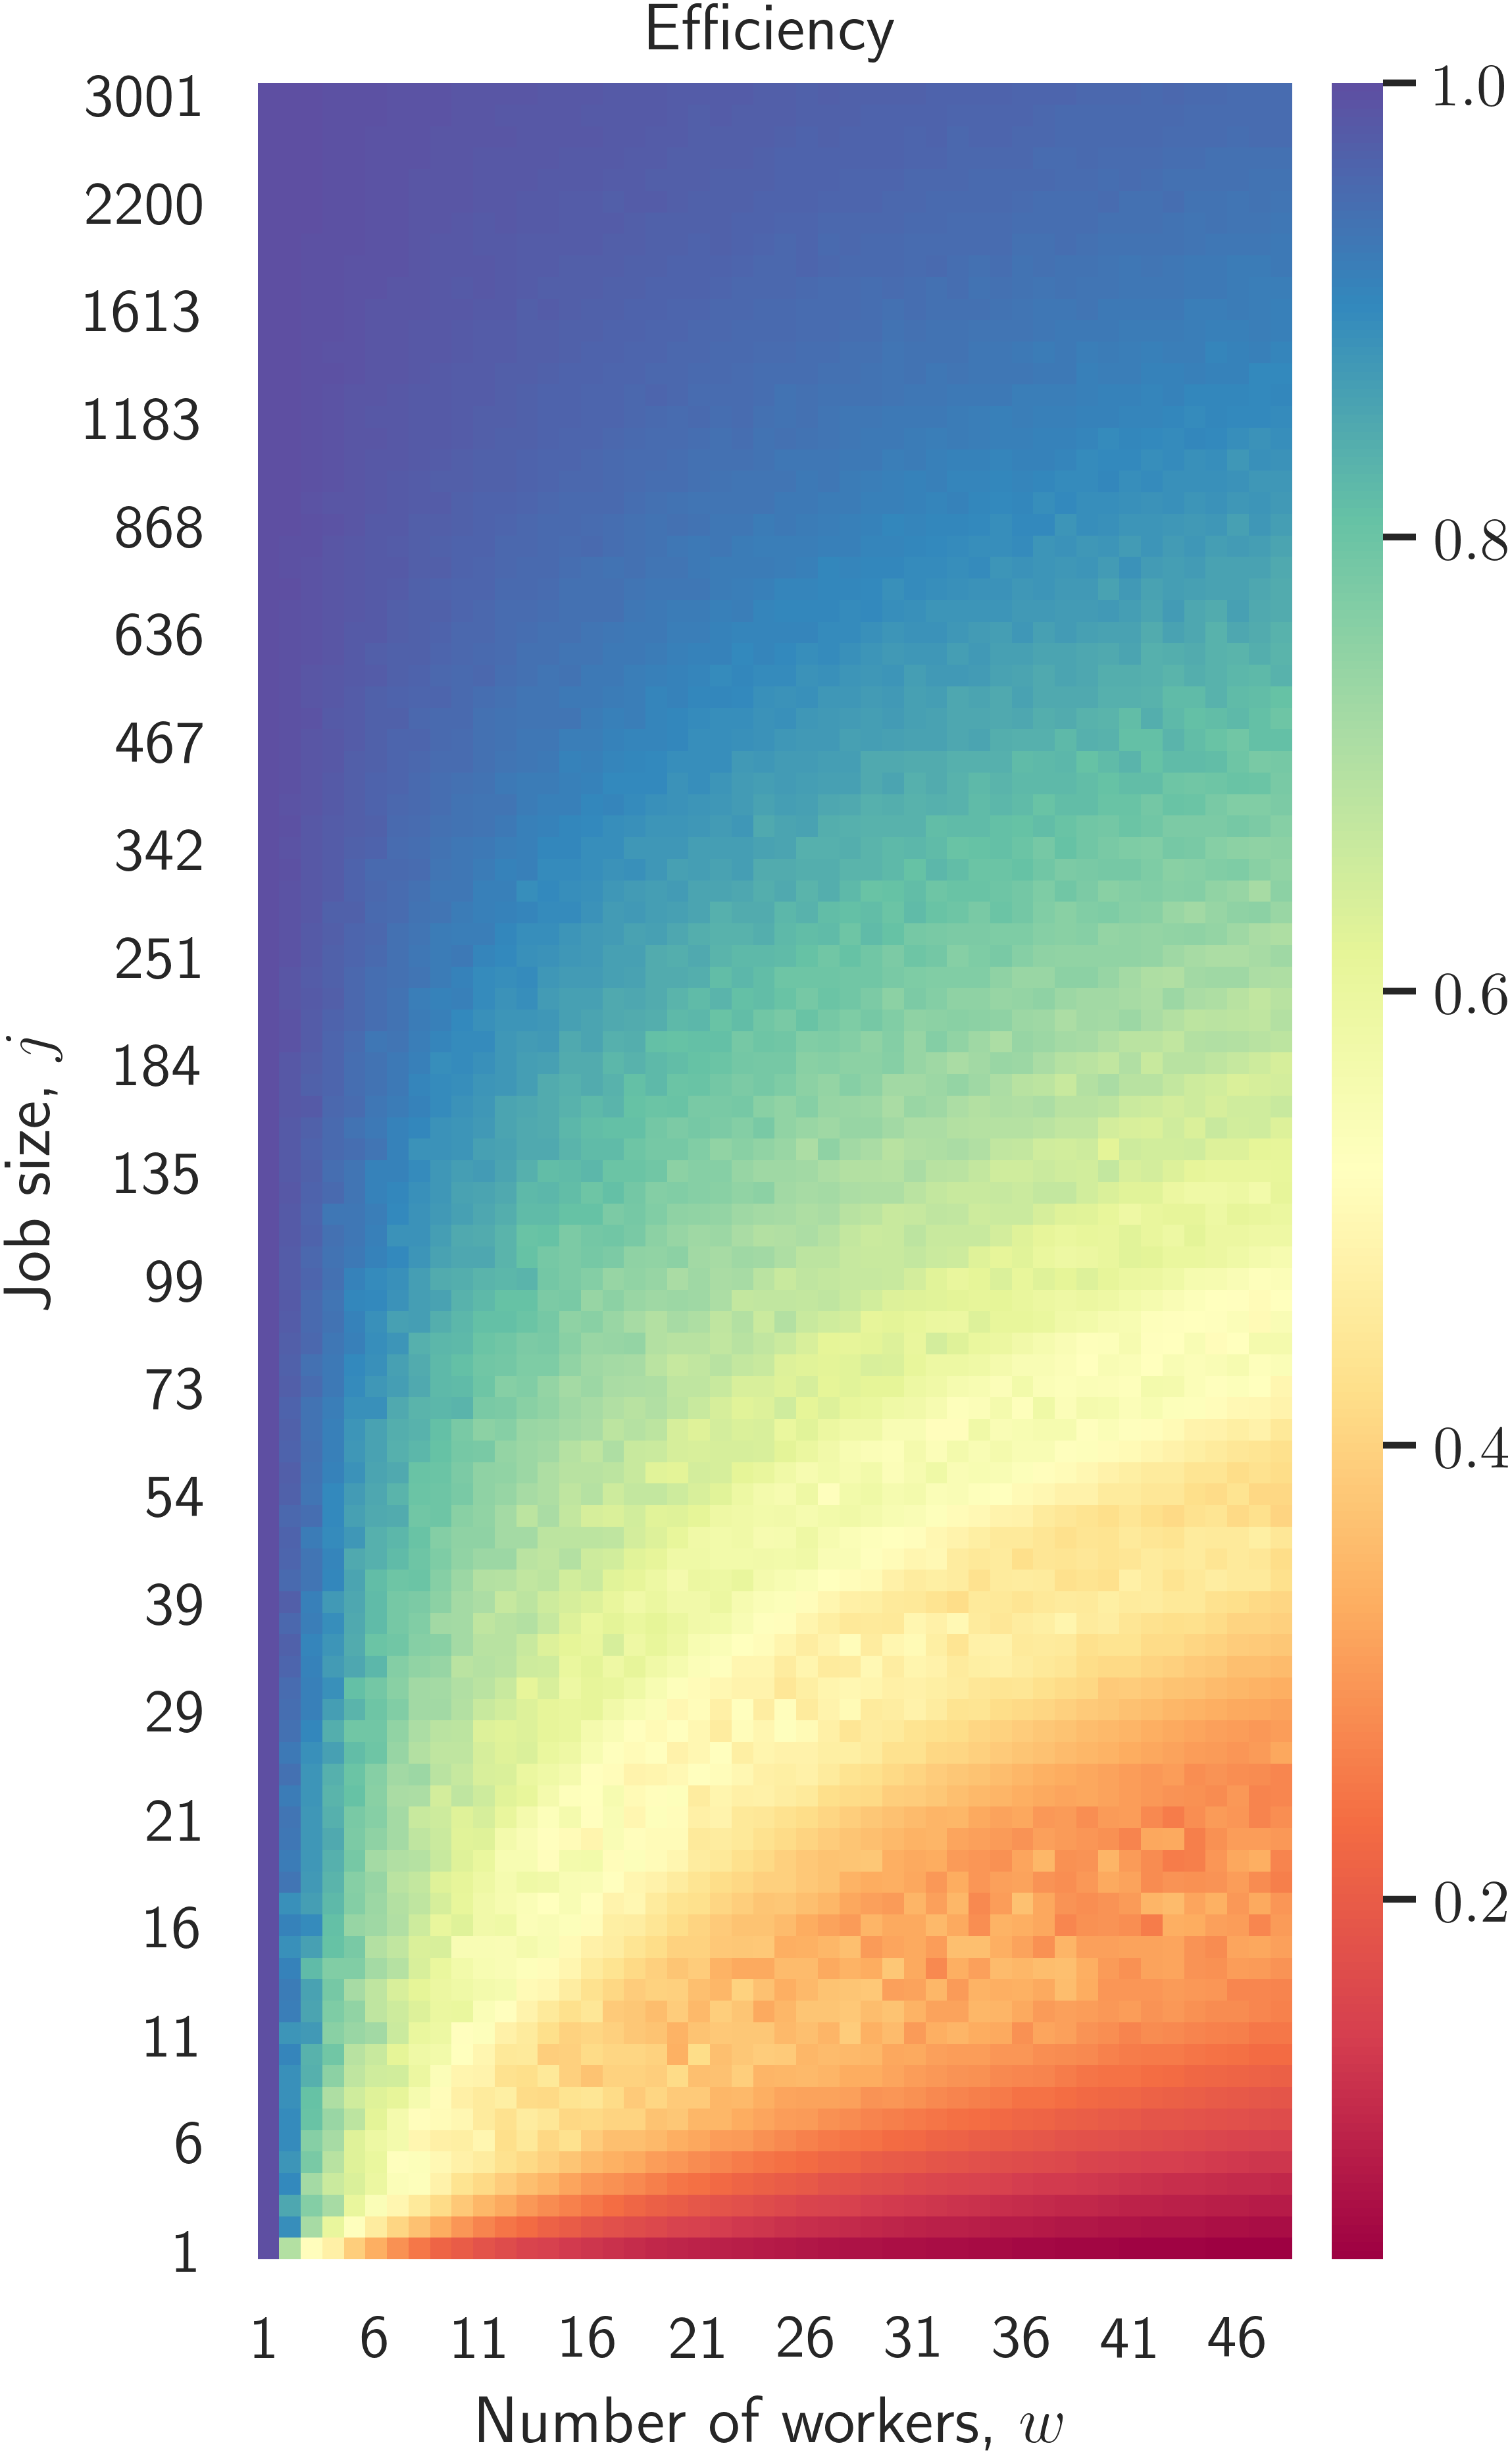
\includegraphics[width=0.36\textwidth]{../assets/worker-efficiency.png}
    \hfill
    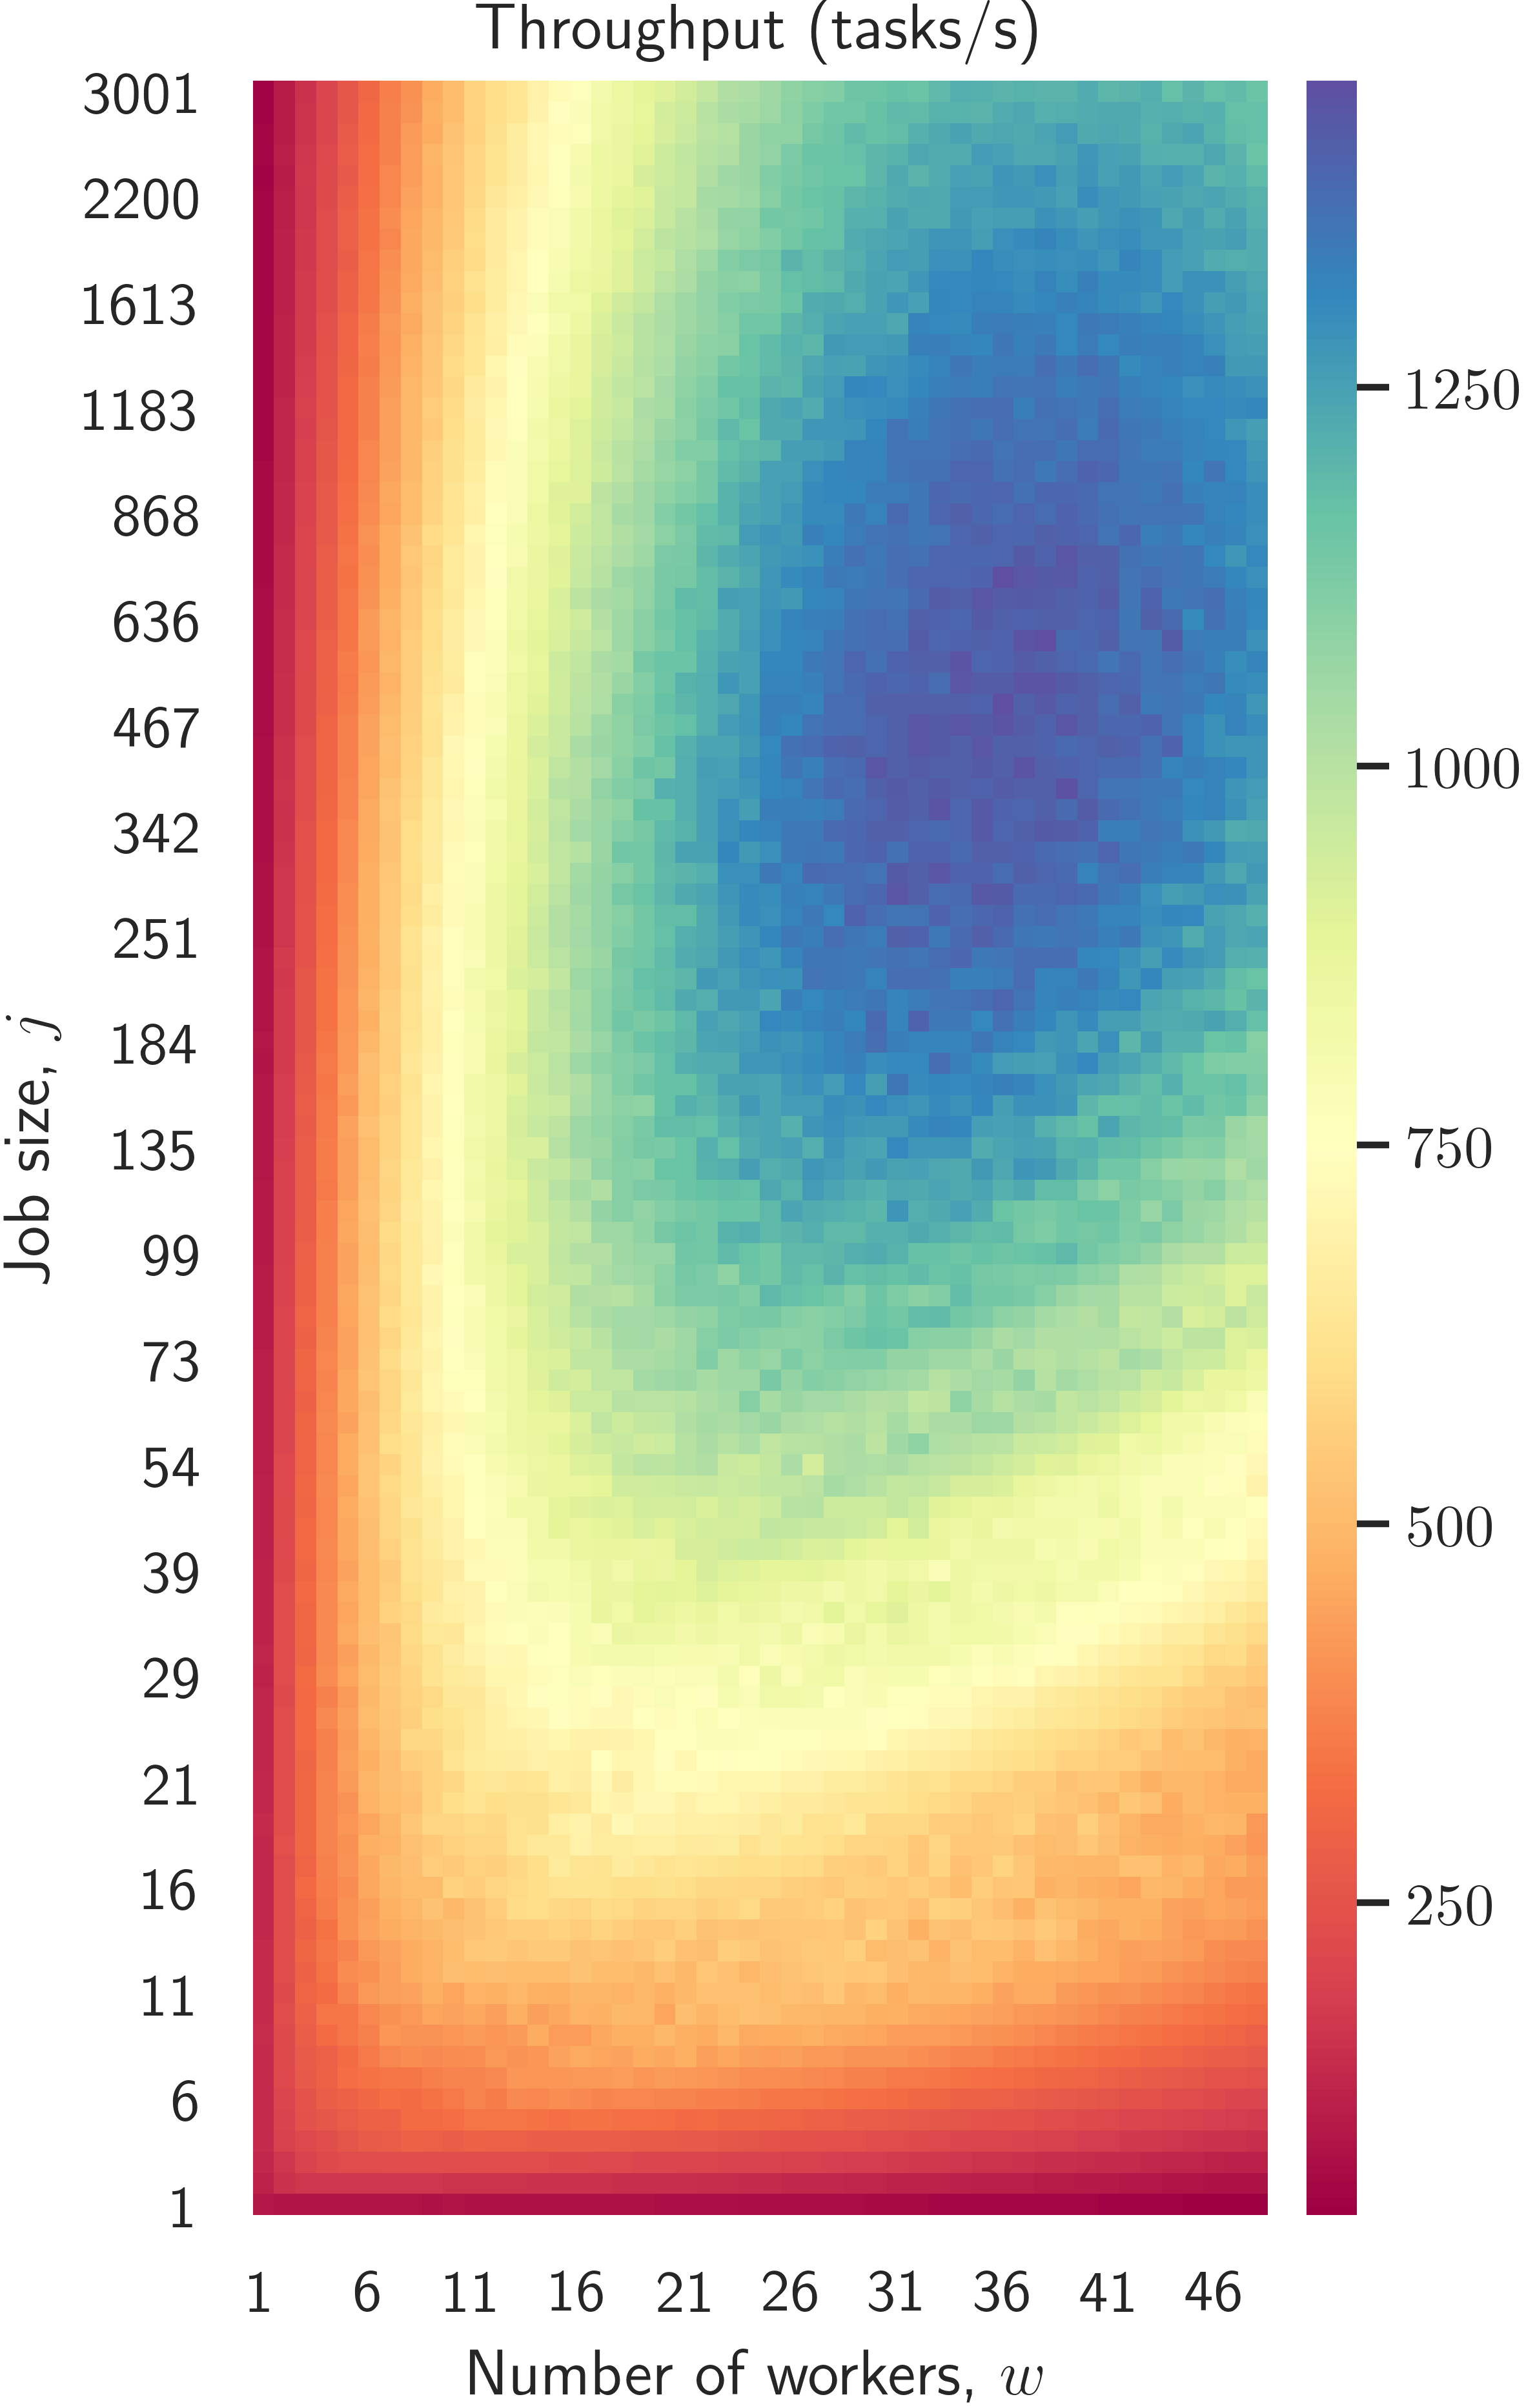
\includegraphics[width=0.36\textwidth]{../assets/worker-throughput.png}
  \end{center}
\end{frame}

% \begin{frame}{Amdahl's Law details}
%   Theoretical latency speedup achievable by a cluster of size $w$ is given by:
%   \[\textsc{speedup}(w) = \left( \frac{s}{s+t} + {t}{w(s+t)} \right)^{-1}\]
%   where $s$ is the (approximately) constant processing time at the server and $t$ is the fixed
%   execution time at the worker.
    
% \end{frame}

\backupend
\end{document}